% =====================================================================
%  Three issues to settle before executing the proposal
%  Reply to "Modularity Matrix Approach for Graph Learning?" (Oct 2026).
%  Self-contained: no .bib, no \includegraphics, no external data.
%  Compiles on Overleaf as-is, and locally with:
%      tectonic -X compile reports/2026-10-18_proposal_issues.tex
%  Every number is printed by modularity_graph_learning/report_numbers.py
% =====================================================================
\documentclass[11pt,a4paper]{article}

\usepackage[T1]{fontenc}
\usepackage[utf8]{inputenc}
\usepackage{lmodern}
\usepackage[margin=2.3cm]{geometry}
\usepackage{amsmath,amssymb,amsthm}
\usepackage{booktabs}
\usepackage{enumitem}
\usepackage{xcolor}
\usepackage{microtype}
\usepackage{caption}
\usepackage{tikz}
\usepackage{pgfplots}
\pgfplotsset{compat=1.18}

\definecolor{BlueLink}{HTML}{1F4E79}
\definecolor{BadRed}{HTML}{B3261E}
\definecolor{LapC}{HTML}{2F6F4E}
\definecolor{Panel2}{HTML}{F7F5F0}
\definecolor{Rule}{HTML}{9AA3AD}

\usepackage[colorlinks=true,linkcolor=BlueLink,urlcolor=BlueLink]{hyperref}
\emergencystretch=3em

\newcommand{\Lap}{\mathbf{L}}
\newcommand{\Wmat}{\mathbf{W}}
\newcommand{\Bmat}{\mathbf{B}}
\newcommand{\Smat}{\mathbf{S}}
\newcommand{\Vmat}{\mathbf{V}}
\newcommand{\dvec}{\mathbf{d}}
\newcommand{\one}{\mathbf{1}}
\newcommand{\tr}{\operatorname{tr}}

\newtheorem{proposition}{Proposition}

\captionsetup{font=small,labelfont=bf,width=.94\textwidth}
\setlist[itemize]{topsep=3pt,itemsep=2pt,parsep=0pt,leftmargin=1.3em}
\setlist[enumerate]{topsep=3pt,itemsep=2pt,parsep=0pt,leftmargin=1.8em}
\setlength{\parskip}{3pt}
\pagestyle{plain}

\newsavebox{\asidebox}
\newenvironment{aside}[1]
 {\par\vspace{2.5mm}\begin{lrbox}{\asidebox}%
  \begin{minipage}{\dimexpr\textwidth-16pt\relax}\small\textbf{#1}\par\vspace{1mm}}
 {\end{minipage}\end{lrbox}%
  \noindent\setlength{\fboxsep}{7pt}\setlength{\fboxrule}{.4pt}%
  \fcolorbox{Rule}{Panel2}{\usebox{\asidebox}}\par\vspace{2.5mm}}

\begin{document}

\begin{center}
{\Large\textbf{Three issues to settle before executing the proposal}}\\[2mm]
{\normalsize Jash Dalal \quad$\cdot$\quad 18 October 2026}\\[1mm]
{\small Reply to \emph{Modularity Matrix Approach for Graph Learning?}\\
Code in \texttt{modularity\_graph\_learning/}; every number below is printed by
\texttt{modularity\_graph\_learning/report\_numbers.py}.}
\end{center}
\vspace{2mm}
\hrule
\vspace{4mm}

% =====================================================================
\section{Summary}
% =====================================================================

While checking the proposal against the code base I found two issues in the proposal
itself and one in our own replication of Paper 1 that Parts I and III depend on.
None of them changes the overall direction; each changes what one task should look
like.

\begin{enumerate}
\item \textbf{Part I(c) does not apply to the paper's time-varying graphs.} The
  identity $\lambda_{\max}(\Bmat_t)=\max\{0,1-\lambda_2(\Lap_t)\}$ needs
  $\operatorname{diag}(\Lap_t)=\one$, and Problem (11) has no degree constraint.
  (Section~\ref{sec:c})
\item \textbf{The Part III objective is unbounded below for every useful $\eta$.} It
  is bounded for $\eta<0.186$ and unbounded for $\eta>0.64$ on our data. The paper
  does not report its $\eta$, but our replication needed $\eta=300$ for the analogous
  Fan term to force three components. Fixing the total edge weight,
  $\one^\top\dvec=p$, appears to repair it without losing convexity.
  (Section~\ref{sec:unbounded})
\item \textbf{Our Fig.~2 replication had not recovered the sectors}, and our SGL
  baseline was not SGL. The first is now fixed (the components are exactly the three
  sectors); the second is relabelled, with a genuine SGL deferred to Part III.
  (Section~\ref{sec:fig2})
\end{enumerate}

% =====================================================================
\section{Part I(c) holds only for unit-degree graphs}\label{sec:c}
% =====================================================================

Parts I(a) and I(b) are correct as stated, and the numerical check on the
$k$-component graph is under way. Part I(c) is also correct as algebra, but it is
applied to the wrong graphs. The paper's time-varying estimator, Problem (11), has
constraint set
\[
  \{\Lap_t\succeq 0,\ \Lap_t\one=\mathbf{0},\ (\Lap_t)_{ij}=(\Lap_t)_{ji}\le 0\},
\]
with no $\operatorname{diag}(\Lap_t)=\one$. That constraint appears only in the
$k$-component problems (6), (8) and (10). Our replication of the time-varying
experiment follows the paper on this point, and its 243 learned FAAMUNG graphs are
far from unit degree:

\begin{center}
\small
\begin{tabular}{lcc}
\toprule
 & mean & range over 243 windows \\
\midrule
mean degree $\bar d$ (Part I needs every $d_i=1$) & 2.13 & [1.51, 2.69] \\
degree coefficient of variation (0 = regular) & 0.305 & [0.240, 0.369] \\
\bottomrule
\end{tabular}
\end{center}

The 8 September report measured the consequence directly: without degree
normalisation, $\Bmat$ and $\Lap$ do not share an eigenbasis on these graphs (mean
best overlap 0.871), and substituting the mean degree into the regular-graph identity
fails. So on the graphs that produce the paper's market indicator,
$\lambda_{\max}(\Bmat_t)$ and $\lambda_2(\Lap_t)$ are different quantities.

Two smaller points. Even on a unit-degree graph, $\max\{0,1-\lambda_2\}$ discards
everything above $\lambda_2=1$; on our series $\lambda_2\ge 1$ in 58\% of windows
(140 of 243), so that indicator would carry no information on most days. What does
survive is a clean reading of the paper's threshold: \emph{if} the graph had unit
degrees, the gate $\lambda_2<\tau=1$ would be exactly Newman's criterion
$\lambda_{\max}(\Bmat)>0$ for the network being divisible at all. I would suggest
stating Part I(c) for unit-degree graphs only, and keeping this observation as a
remark.

% =====================================================================
\section{The Part III objective is unbounded below}\label{sec:unbounded}
% =====================================================================

The proposed objective is
$f(\Wmat)=\tr(\Lap\Smat)-\log\operatorname{gdet}(\Lap)-\eta\,\tr(\Vmat^\top\Bmat(\Wmat)\Vmat)$.
Its first and last terms are homogeneous of degree one in the edge weights, and only
the log term resists scale. Along any ray $\Wmat=c\,\Wmat_0$, with $\Vmat$ chosen
optimally (the top $k-1$ eigenvectors of $\Bmat$, which do not move with $c$),
\[
  f(c\,\Wmat_0)\;=\;c\,(a-\eta b)\;-\;r\log c\;+\;\text{const},\qquad
  a=\tr(\Lap_0\Smat),\quad b=\textstyle\sum_{i<k}\mu_i(\Bmat_0),\quad r=\operatorname{rank}\Lap_0 .
\]
If $\eta b>a$ for any feasible $\Wmat_0$, then $f\to-\infty$ as $c\to\infty$. The
paper's own Fan term does not have this problem, because
$\eta\tr(\Vmat^\top\Lap\Vmat)\ge 0$; the modularity term can be positive.

\begin{proposition}
Let $Z_{ij}=S_{ii}+S_{jj}-2S_{ij}$ and $Z_{\min}=\min_{i\neq j}Z_{ij}$. The
objective is bounded below whenever $\eta<Z_{\min}/(k-1)$.
\end{proposition}
\begin{proof}[Sketch]
Write $m=\sum_{i<j}W_{ij}$. Then $\tr(\Lap\Smat)=\sum_{i<j}W_{ij}Z_{ij}\ge Z_{\min}m$.
Since $\Bmat\preceq\Wmat$, each eigenvalue of $\Bmat$ is at most
$\lambda_{\max}(\Wmat)\le d_{\max}\le m$, so the modularity term is at most $(k-1)m$.
Hence $f\ge(Z_{\min}-\eta(k-1))\,m-r\log(2m/r)$, which is bounded below in $m$.
\end{proof}

On the other side, the worst graph I have found puts all weight on the $k$ most
correlated disjoint pairs. Then $\Bmat_0$ has eigenvalue $w$ with multiplicity $k-1$,
so $b=(k-1)w$ while $a=w\sum Z$, which is small. The table gives the thresholds on
the 753-day data ($p=97$, $k=3$). The connected variant adds a complete graph of
weight $10^{-6}$, so the conclusion does not depend on how $\operatorname{gdet}$
treats disconnected graphs.

\begin{center}
\small
\begin{tabular}{lccc}
\toprule
ray $\Wmat_0$ & $a$ & $b$ & unbounded once $\eta>a/b$ \\
\midrule
ideal sector graph (unit degree, complete inside sectors) & 56.691 & 2.000 & 28.35 \\
Problem (1) estimate, $\beta=0$ & 96.000 & 5.162 & 18.60 \\
3 disjoint pairs (RSG/WM, DAL/UAL, LMT/NOC) & 1.280 & 2.000 & 0.64 \\
\quad same, plus $10^{-6}$ complete graph (connected) & 1.287 & 2.000 & 0.64 \\
\midrule
\multicolumn{3}{l}{bounded for $\eta<Z_{\min}/(k-1)$, with $Z_{\min}=0.373$ (RSG/WM)} & 0.186 \\
\bottomrule
\end{tabular}
\end{center}

\begin{figure}[h]
\centering
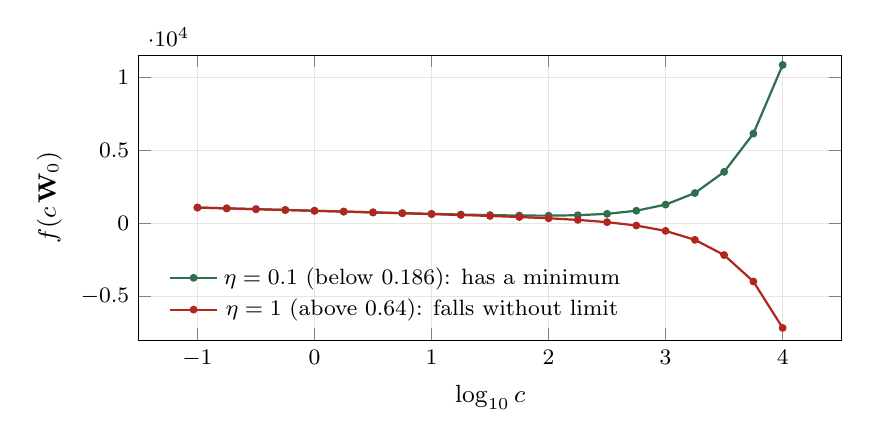
\begin{tikzpicture}
\begin{axis}[width=10.5cm,height=5.2cm,xlabel={$\log_{10} c$},ylabel={$f(c\,\Wmat_0)$},
  legend pos=south west,legend style={font=\footnotesize,draw=none,fill=none},
  tick label style={font=\footnotesize},label style={font=\small},
  ymin=-8000,ymax=11500,grid=major,grid style={gray!20}]
\addplot[LapC,thick,mark=*,mark size=1pt] coordinates {
(-1.00,1078.5) (-0.75,1023.3) (-0.50,968.2) (-0.25,913.2) (0.00,858.4) (0.25,804.0) (0.50,750.2) (0.75,697.6) (1.00,647.1) (1.25,600.3) (1.50,560.1) (1.75,531.6) (2.00,523.9) (2.25,553.2) (2.50,648.3) (2.75,860.5) (3.00,1280.8) (3.25,2071.3) (3.50,3519.9) (3.75,6139.0) (4.00,10839.6)};
\addlegendentry{$\eta=0.1$ (below 0.186): has a minimum}
\addplot[BadRed,thick,mark=*,mark size=1pt] coordinates {
(-1.00,1078.3) (-0.75,1023.0) (-0.50,967.6) (-0.25,912.2) (0.00,856.6) (0.25,800.8) (0.50,744.5) (0.75,687.5) (1.00,629.1) (1.25,568.3) (1.50,503.2) (1.75,430.4) (2.00,343.9) (2.25,233.1) (2.50,79.1) (2.75,-151.7) (3.00,-519.2) (3.25,-1129.6) (3.50,-2172.2) (3.75,-3983.1) (4.00,-7160.4)};
\addlegendentry{$\eta=1$ (above 0.64): falls without limit}
\end{axis}
\end{tikzpicture}
\caption{The Part III objective along the connected three-pairs ray. Scaling every
edge weight by $c$ lowers it without limit once $\eta$ exceeds the ray's threshold.}
\end{figure}

\textbf{What the modularity term rewards.} Expanding with $\Wmat=\mathbf{D}-\Lap$
gives an identity (checked to $1.7\times10^{-15}$):
\[
  -\tr(\Vmat^\top\Bmat\Vmat)\;=\;\tr(\Vmat^\top\Lap\Vmat)\;-\;\sum_i d_i\,\lVert v_i-c_d\rVert^2,
  \qquad c_d=\frac{\Vmat^\top\dvec}{\one^\top\dvec},
\]
where $v_i$ is row $i$ of $\Vmat$. The prior is the paper's Fan term minus a reward
for placing degree on nodes whose embedding is far from the degree-weighted centre.
With unit degrees and $\Vmat\perp\one$ the reward is the constant $k-1$, which
recovers Part I(b). The reward grows linearly with scale, which is the source of the
unboundedness. It also bears on the isolated-node question: a node with $d_i=0$
forfeits its share of the reward, so the term discourages isolation rather than
merely failing to prevent it.

\begin{aside}{A possible repair}
One way to settle this would be to keep only the weakest part of the paper's degree
constraint: fix the total weight, $\one^\top\dvec=p$ (average degree one), and drop
$\operatorname{diag}(\Lap)=\one$. The constraint is linear, so the $\Lap$-subproblem
stays convex; the feasible edge weights become a compact simplex, so the objective is
bounded for every $\eta$; the quadratic-over-linear term becomes the plain quadratic
$\lVert\Vmat^\top\dvec\rVert^2/p$; and individual degrees are still free to differ.
It reduces to the paper's normalisation when every $d_i=1$. The scale-free
alternative, normalised modularity $\tr(\Vmat^\top\Bmat\Vmat)/\one^\top\dvec$, would
also remove the problem but gives up convexity. Which repair fits the intent of Part
III is your call.
\end{aside}

% =====================================================================
\section{Our Fig.~2 replication}\label{sec:fig2}
% =====================================================================

The Part I numerical check needs a $k$-component graph whose components mean
something, so I re-examined our Fig.~2 first. Our replication had marked it as
reproduced because Algorithm 1 returned three components (rank $p-3$). It had not
checked what the components were, and they were not the sectors.

\textbf{Two causes.} The data window was four years (1{,}005 days) instead of the
paper's three (753); that is now fixed. The larger cause was the starting point. Our
Algorithm 1 started from the uniform complete graph, whose nonzero Laplacian
eigenvalue $p/(p-1)$ has multiplicity $p-1$. The first $\Vmat$-step therefore picks an
arbitrary basis of that eigenspace, and the components the spectral penalty then
forces are arbitrary too: they are set by floating-point round-off. Changing nothing
but the number of BLAS threads changes the answer. Starting instead from the Problem
(1) estimate (the paper's Algorithm 1 does take an initial estimate $\Lap_0$) gives
the sectors exactly, and the answer no longer depends on round-off.

\begin{center}
\small
\begin{tabular}{llllc}
\toprule
start & window & BLAS threads & components (sizes) & ARI vs sectors \\
\midrule
uniform & 1{,}005 days & default & 77 / 12 / 8 & 0.012 \\
uniform & 753 days & 1 & 96 + 1 isolated node & $-0.009$ \\
uniform & 753 days & default & 93 / 2 / 2 & $-0.020$ \\
Problem (1) & 753 days & 1 & 52 / 28 / 17 & 1.000 \\
Problem (1) & 753 days & default & 52 / 28 / 17 & 1.000 \\
\bottomrule
\end{tabular}
\end{center}

The sector sizes are 52, 28 and 17, so ARI 1.000 means the components are exactly the
Industrials, Consumer Staples and Energy stocks. The two Problem (1) runs differ by at
most $7.7\times10^{-5}$ in any entry of $\Lap$; the two uniform runs differ by 1.0, the size of the entries themselves.
For reference, $k$-means on the top three eigenvectors of the correlation matrix itself scores 0.900.

One uniform run also left a stock with degree exactly zero, despite the degree penalty. Neither the soft constraint $\operatorname{diag}(\Lap)\approx\one$ nor the $\log\operatorname{gdet}$ term rules isolation out: the solver can set a whole row of weights to zero in one projected step, after which that eigenvalue simply leaves the pseudo-determinant. This bears on Part III, since isolated nodes can come from the alternating scheme's starting point as well as from missing degree control.

Two related corrections. Our ``SGL'' baseline was Problem (1) with an $\ell_1$
penalty and no spectral constraint, so the figure never tested the paper's claim that
spectral constraints without degree control yield isolated nodes; it is now labelled
as what it is, and a genuine SGL is deferred to Part III. And our Fig.~1 matches the
paper's ranking only narrowly: correlation with the market kept puts 199 of its 200
strongest edges inside a sector, against 198 with the market removed. A small gap is
consistent with the invariance $\tr(\Lap\Smat)=\tr(\Lap\mathbf{J}\Smat\mathbf{J})$
behind Part II, though our market removal regresses each stock on the equal-weighted
mean, so it is not exactly the uniform direction that invariance discards.

% =====================================================================
\section{Suggested next steps}
% =====================================================================

I would suggest the following order, though it is a judgement call. With Fig.~2
repaired, the Part I numerical check can now run on a $k$-component graph whose
components mean something. Next would be Part I as the short expository note, with (c) restricted to unit-degree graphs and the
normalised-operator case placed as the general statement (it is the 8 September
identity, of which Part I is the special case $\mathbf{u}=\one/\sqrt p$). Parts II
and III could follow once you have decided on the Part III repair; Part III will also
need a genuine SGL implementation, which I would write in Python since the reference
implementation is an R package.

\end{document}
